\documentclass{beamer}

\mode<presentation>
{
	\usetheme{CambridgeUS}
	\setbeamercovered{transparent}
}

\setbeamertemplate{caption}[numbered]

\usepackage[spanish]{babel}
\usepackage[latin1]{inputenc}
\usepackage{color}
\usepackage{multicol}
\usepackage{hyperref}
\usepackage{algorithm,algorithmic}
\usepackage{colortbl}
\usepackage{graphicx}

\title[\textbf{Programaci\'on 2}]{\textbf{Programaci\'on 2}}

\subtitle{Lenguaje Java - \emph{Threads (Hilos)}}

\author[Rodrigo Olivares]
{
	Rodrigo Olivares \\
	\vspace{0.5mm}
	Mg. en Ingenier\'ia Inform\'atica \\
	\vspace{0.5mm}
	\texttt{\normalsize rodrigo.olivares@uv.cl}
}

\institute[Universidad de Valpara\'iso]

\date{$2^{do}$ Semestre de 2016} 

\subject{Programaci\'on 2}

\AtBeginSection
{
	\begin{frame}<beamer>
	\frametitle{Contenido}
	\tableofcontents[currentsection,currentsubsection]
	\end{frame}
}

\AtBeginSubsection
{
	\begin{frame}<beamer>
	\frametitle{Contenido}
	\tableofcontents[currentsection,currentsubsection]
	\end{frame}
}

\beamerdefaultoverlayspecification{<+->}

\begin{document}

	\begin{frame}
		\titlepage
	\end{frame}

	\begin{frame}
		\frametitle{Contenido}
		\tableofcontents[pausesections]
	\end{frame}

    \section{Threads}

    \subsection{Introducci\'on}

	\begin{frame}
		\frametitle{Threads}
		\framesubtitle{Introducci\'on}

		\begin{block}{Introducci\'on}
			Los procesadores y los Sistemas Operativos modernos permiten la \textbf{multitarea}, es decir, la realizaci\'on simult\'anea de dos o m\'as actividades (\emph{al menos aparentemente})
		\end{block}
	\end{frame}

    	\begin{frame}
		\frametitle{Threads}
		\framesubtitle{Introducci\'on}

		En ordenadores con dos o m\'as procesadores, la \textbf{multitarea es real}, ya que cada procesador puede ejecutar un \textbf{hilo} o \textbf{thread} diferente.
        \begin{center}
            \begin{figure}
        			\fbox{\fbox{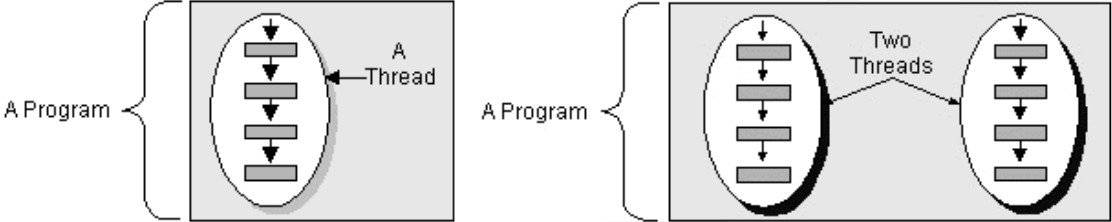
\includegraphics[width=11.5cm]{images/threads.png}}}
                \caption{Programa con 1 y con 2 threads o hilos.}
            \end{figure}
		\end{center}
	\end{frame} 
	
	\begin{frame}
		\frametitle{Threads}
		\framesubtitle{Introducci\'on}

		\begin{alertblock}{Proceso y thread}
			Un proceso es un \textbf{programa} ejecut\'andose de forma independiente y con un espacio propio de memoria. Un thread o hilo es un \textbf{flujo secuencial} simple dentro de un proceso. Un \'unico proceso puede tener varios hilos ejecut\'andose.
        \end{alertblock}
        \begin{exampleblock}{Ejemplo}
			Un claro ejemplo de un proceso ser\'ian algunos navegadores web, como Google Chrome y Mozilla Firefox. Cada pesta\~na ejecut\'andose ser\'ia un hilo o threads del proceso.
        \end{exampleblock}
	\end{frame} 

    \begin{frame}
		\frametitle{Threads}
		\framesubtitle{Introducci\'on}

		\begin{alertblock}{Proceso y thread}
			Un sistema multitarea da realmente la impresi\'on de estar haciendo varias cosas a la vez y eso es una gran ventaja para el usuario.
        \end{alertblock}
		\begin{alertblock}{}        
			Sin el uso de threads hay tareas que son pr\'acticamente imposibles de ejecutar, particularmente las que tienen tiempos de espera importantes entre etapas.
        \end{alertblock}
	\end{frame} 

    \begin{frame}
		\frametitle{Threads}
		\framesubtitle{Introducci\'on}

		\begin{alertblock}{Proceso y thread}
			Los threads o hilos de ejecuci\'on permiten organizar los recursos del ordenador de forma que pueda haber varios programas actuando en paralelo. Un hilo de ejecuci\'on puede realizar cualquier tarea que pueda realizar un programa com\'un y corriente. Bastar\'a con indicar lo que tiene que hacer en el m\'etodo \textbf{run}(), que es el que define la actividad principal de las threads.
        \end{alertblock}
	\end{frame} 

    \begin{frame}
		\frametitle{Threads}
		\framesubtitle{Introducci\'on}

		\begin{alertblock}{Proceso y thread}
			Los threads pueden ser \textbf{daemon} o \textbf{no daemon}. Son \textbf{daemon} aquellos hilos que realizan en \textbf{background} (en un segundo plano) servicios generales. Esto es, tareas que no forman parte de la esencia del programa y que se est\'an ejecutando mientras no finalice la aplicaci\'on. Un thread \textbf{daemon} podr\'ia ser por ejemplo aqu\'el que est\'a comprobando permanentemente si el usuario pulsa un bot\'on. Un programa de Java finaliza cuando s\'olo quedan corriendo threads de tipo daemon. Por defecto, y si no se indica lo contrario, los threads son del tipo \textbf{no daemon}.
        \end{alertblock}
	\end{frame}

    \subsection{Creaci\'on de threads}

	\begin{frame}
		\frametitle{Threads}
		\framesubtitle{Creaci\'on de threads}

		\begin{block}{Creaci\'on}
            En Java hay \textbf{dos} formas de crear nuevos threads:
            \begin{itemize}
                \item[$\rightarrow$] Crear una nueva clase hija que \textbf{herede} de la clase padre \textbf{java.lang.Thread} y sobrecargar el m\'etodo \textbf{run}() de dicha clase.
                \item[$\rightarrow$] Declarar una clase que implemente la \emph{interface} \textbf{java.lang.Runnable}, la cual declarar\'a el m\'etodo \textbf{run}(); posteriormente se crea un objeto de tipo \textbf{Thread} pas\'andole como argumento en el constructor, el objeto creado de la nueva clase (la que implementa la interface \textbf{Runnable})
            \end{itemize}
        \end{block}
        \begin{block}{}
            Como ya se ha apuntado, tanto la clase \textbf{Thread} como la interface \textbf{Runnable} pertenecen al package \textbf{java.lang}, por lo que no es necesario importarlas.
        \end{block}
	\end{frame}
	
	\begin{frame}
		\frametitle{Threads}
		\framesubtitle{Creaci\'on de threads}

		\begin{block}{Ejemplo, Creaci\'on de threads derivando de la clase Thread}
            \textbf{public class} SimpleThread \textbf{extends Thread} \{ \\
            \hspace*{10pt}\textcolor{gray}{// constructor} \\
            \hspace*{10pt}\textbf{public} SimpleThread (String str) \{ \\
            \hspace*{20pt}super(str);\\
            \hspace*{10pt}\} \\ ~\\
            \hspace*{10pt}\textcolor{gray}{// redefinici\'on del m\'etodo run()}\\
            \hspace*{10pt}\textbf{public void} run() \{\\
            \hspace*{20pt}\textbf{for}(\textbf{int} i = 0; i $<$ 10; i$++$) \{\\
            \hspace*{30pt}System.out.println(''Este es el thread : '' + getName());\\
            \hspace*{20pt}\} \\
            \hspace*{10pt}\} \\
            \}
        \end{block}
	\end{frame}
	
	\begin{frame}
		\frametitle{Threads}
		\framesubtitle{Creaci\'on de threads}

		\begin{block}{Ejemplo, Creaci\'on de threads derivando de la clase Thread}
            En este caso, se ha creado la clase \textbf{SimpleThread}, que hereda de \textbf{Thread}. En su constructor se utiliza un \textbf{String} (opcional) para poner nombre al nuevo \textbf{thread} creado, y mediante \textbf{super}() se llama al constructor de la super-clase \textbf{Thread}. Asimismo, se redefine el m\'etodo \textbf{run}(), que define la principal actividad del thread, para que escriba 10 veces el nombre del thread creado.
        \end{block}
	\end{frame}	
	
	\begin{frame}
		\frametitle{Threads}
		\framesubtitle{Creaci\'on de threads}

        \begin{block}{Ejemplo, Creaci\'on de threads derivando de la clase Thread}
            Para poner en marcha este nuevo \textbf{thread} se debe crear un objeto de la clase \textbf{SimpleThread}, y llamar al m\'etodo start(), heredado de la super-clase \textbf{Thread}, que se encarga de llamar a \textbf{run}(). Por ejemplo:
            \begin{itemize}
                \item[] \textbf{SimpleThread} miThread = \textbf{new SimpleThread}(''Hilo de prueba'');
                \item[] miThread.\emph{start}();
            \end{itemize}
        \end{block}
	\end{frame}		
	
	\begin{frame}
		\frametitle{Threads}
		\framesubtitle{Creaci\'on de threads}

		\begin{block}{Ejemplo, Creaci\'on de threads implementando la interface Runnable}
            Esta segunda forma tambi\'en requiere que se defina el m\'etodo run(), pero adem\'as es necesario crear un objeto de la clase \textbf{Thread} para lanzar la ejecuci\'on del nuevo hilo. Al constructor de la clase \textbf{Thread} hay que pasarle una referencia del objeto de la clase que implementa la interface Runnable. Posteriormente, cuando se ejecute el m\'etodo \textbf{start}() del thread, \'este llamar\'a al m\'etodo run() definido en la nueva clase.
        \end{block}
	\end{frame}

	\begin{frame}
		\frametitle{Threads}
		\framesubtitle{Creaci\'on de threads}

		\begin{block}{Ejemplo, Creaci\'on de threads implementando la interface Runnable}
        		\textbf{public class} SimpleRunnable \textbf{implements Runnable} \{ \\        
            \hspace*{10pt}\textcolor{gray}{// se crea un nombre} \\
            \hspace*{10pt}\textbf{String} nameThread; \\
            \hspace*{10pt}\textbf{public} SimpleRunnable (String str) \{ \\
            \hspace*{20pt}nameThread = str;\\
            \hspace*{10pt}\} \\ ~\\
            \hspace*{10pt}\textcolor{gray}{// definici\'on del m\'etodo run()}\\
            \hspace*{10pt}\textbf{public void} run() \{\\
            \hspace*{20pt}\textbf{for}(\textbf{int} i = 0; i $<$ 10; i$++$) \{\\
            \hspace*{30pt}System.out.println(''Este es el thread : '' + nameThread);\\
            \hspace*{20pt}\} \\
            \hspace*{10pt}\} \\
            \}
        \end{block}
	\end{frame}
	
	\begin{frame}
		\frametitle{Threads}
		\framesubtitle{Creaci\'on de threads}

        \begin{block}{Ejemplo, Creaci\'on de threads implementando la interface Runnable}
            El siguiente c\'odigo crea un nuevo thread y lo ejecuta el segundo procedimiento:
            \begin{itemize}
                \item[] \textbf{SimpleRunnable} miRunnable = \textbf{new SimpleRunnable}(''Hilo de prueba'');
                \item[] \textbf{Thread} miThread = new \textbf{Thread}(miRunnable);
                \item[] miThread.\emph{start}();
            \end{itemize}
        \end{block}
	\end{frame}
	
	\begin{frame}
		\frametitle{Threads}
		\framesubtitle{Creaci\'on de threads}

        \begin{alertblock}{Elecci\'on \textquestiondown Thread o Runnable?}
            La elecci\'on de una u otra forma depende del tipo de clase que se vaya a crear. As\'i, si la clase a utilizar ya hereda de otra clase, no quedar\'a m\'as que implementar \textbf{Runnable}, aunque normalmente es m\'as ''sencillo'' heredar de \textbf{Thread}.
        \end{alertblock}
	\end{frame}	

    \subsection{Ciclo de vida de un thread}

	\begin{frame}
		\frametitle{Threads}
		\framesubtitle{Ciclo de vida de un thread}

        En la secci\'on anterior se ha visto c\'omo crear nuevos objetos que permiten incorporar en un programa la posibilidad de realizar varias tareas simult\'aneamente. En la Figura \ref{fig-ciclo} se muestran los distintos estados por los que puede pasar un thread a lo largo de su vida. 
        \begin{center}
            \begin{figure}
                \fbox{\fbox{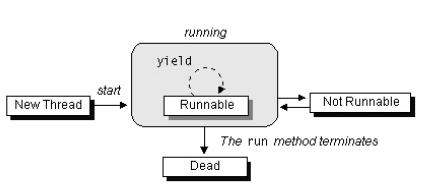
\includegraphics[width=8cm]{images/ciclo.png}}}
                \caption{Ciclo de vida de un Thread.}\label{fig-ciclo}
            \end{figure}
	    \end{center}
	\end{frame}	

	\begin{frame}
		\frametitle{Threads}
		\framesubtitle{Ciclo de vida de un thread}

        \begin{block}{Ciclo de vida de un thread}
            {\scriptsize
            Un \textbf{thread} puede presentar \textbf{cuatro} estados distintos:
            \begin{enumerate}
                \item Nuevo (\textbf{New}): El thread ha sido creado pero no inicializado, es decir, no se ha ejecutado el m\'etodo \textbf{start}() (\textbf{IllegalThreadStateException}). 
                \item Ejecutable (\textbf{Runnable}): El thread puede estar ejecut\'andose, siempre y cuando se le haya asignado un determinado tiempo de CPU. En la pr\'actica puede no estar siendo ejecutado en un instante determinado, en beneficio de otro \textbf{thread}.
                \item Bloqueado (\textbf{Blocked} o \textbf{Not Runnable}): El thread podr\'ia estar ejecut\'andose, pero hay alguna actividad interna suya que lo impide, como por ejemplo una espera producida por una operaci\'on de escritura o lectura de datos por teclado (E/S). Si un thread est\'a en este estado, no se le asigna tiempo de CPU.
                \item Muerto (\textbf{Dead}): La forma habitual de que un \textbf{thread} muera es finalizando el m\'etodo \textbf{run}(). Tambi\'en puede llamarse al m\'etodo \textbf{stop}() de la clase \textbf{Thread}, aunque dicho m\'etodo es considerado ''peligroso'' y no se debe utilizar.
            \end{enumerate}
            }
        \end{block}
	\end{frame}	

    \subsection{Sincronizaci\'on}

	\begin{frame}
		\frametitle{Threads}
		\framesubtitle{Sincronizaci\'on}

        \begin{block}{Sincronizaci\'on}
            La \textbf{sincronizaci\'on} nace de la necesidad de evitar que dos o m\'as \textbf{threads} traten de acceder a los mismos recursos al mismo tiempo.
        \end{block}
        \begin{exampleblock}{Caso}
            As\'i, por ejemplo, si un \textbf{thread} tratara de escribir en un fichero y otro thread estuviera al mismo tiempo tratando de borrar dicho fichero, se producir\'ia una situaci\'on
no deseada.
        \end{exampleblock}
	\end{frame}

	\begin{frame}
		\frametitle{Threads}
		\framesubtitle{Sincronizaci\'on}

        \begin{alertblock}{Secciones cr\'iticas}
            Las secciones de c\'odigo de un programa que acceden a un mismo recurso (un mismo objeto de una clase, un fichero del disco, etc.) desde dos \textbf{threads} distintos se denominan secciones cr\'iticas (\textbf{critical sections}).
        \end{alertblock}
        \begin{block}{Sincronizar}
            Para sincronizar dos o m\'as \textbf{threads}, hay que utilizar el modificador \textbf{synchronized} en aquellos m\'etodos del \textbf{objeto-recurso} con los que puedan producirse situaciones conflictivas. De esta forma, Java bloquea (asocia un bloqueo o \textbf{lock}) con el recurso sincronizado.
        \end{block}
	\end{frame}

    \begin{frame}
		\frametitle{Threads}
		\framesubtitle{Sincronizaci\'on}

        \begin{block}{Sincronizar}
            La sincronizaci\'on previene las interferencias solamente sobre un tipo de recurso: la memoria reservada para un objeto. Cuando se prevea que unas determinadas variables de una clase pueden tener problemas de sincronizaci\'on, se deber\'an declarar como \textbf{private} (o \textbf{protected}). De esta forma s\'olo estar\'an accesibles a trav\'es de m\'etodos de la clase, que deber\'an estar sincronizados.
        \end{block}
	\end{frame}

    \begin{frame}
		\frametitle{Threads}
		\framesubtitle{Sincronizaci\'on}

        \begin{block}{Sincronizar}
            Es muy importante tener en cuenta que si se sincronizan algunos m\'etodos de un objeto, pero otros no, el programa puede \textbf{no funcionar correctamente}. La raz\'on es que los m\'etodos \textbf{no sincronizados} pueden acceder libremente a las variables miembro, ignorando el \textbf{bloqueo del objeto}. S\'olo los m\'etodos sincronizados comprueban si un objeto est\'a bloqueado. Por lo tanto, todos los m\'etodos que accedan a un recurso compartido deben ser declarados \textbf{synchronized}.
        \end{block}
         \begin{block}{Sincronizar - Niveles de bloqueo} 
            Existen dos niveles de bloqueo de un recurso. El primero es a \textbf{nivel de objetos}, mientras que el segundo es a \textbf{nivel de clases}.
        \end{block}
	\end{frame}

    \begin{frame}
		\frametitle{Threads}
		\framesubtitle{Sincronizaci\'on}

        \begin{block}{Sincronizar - Niveles de bloqueo - A nivel de objeto} 
            Se consigue declarando todos los m\'etodos de una clase como \textbf{synchronized}. Cuando se ejecuta un m\'etodo \textbf{synchronized} sobre un objeto concreto, el sistema bloquea dicho objeto, de forma que si otro \textbf{thread} intenta ejecutar alg\'un m\'etodo sincronizado de ese objeto, este segundo m\'etodo se mantendr\'a a la espera hasta que finalice el anterior (y desbloquee por lo tanto el objeto).
        \end{block}
	\end{frame}

    \begin{frame}
		\frametitle{Threads}
		\framesubtitle{Sincronizaci\'on}

        \begin{block}{Sincronizar - Niveles de bloqueo - A nivel de clases} 
            Corresponde al bloqueo de los \textbf{m\'etodos de clase} o \textbf{static}, y por lo tanto con las \textbf{variables de clase} o \textbf{static}. Si lo que se desea es conseguir que un m\'etodo bloquee simult\'aneamente una clase entera, es decir todos los objetos creados de una clase, es necesario declarar este m\'etodo como \textbf{synchronized static}.
        \end{block}
	\end{frame}

    \subsection{Prioridades}
    
    \begin{frame}
		\frametitle{Threads}
		\framesubtitle{Prioridades}

        \begin{block}{Prioridades} 
            Con el fin de conseguir una correcta ejecuci\'on de un programa se establecen prioridades en los threads, de forma que se produzca un reparto m\'as eficiente de los recursos disponibles.
        \end{block}
        \begin{block}{Caso} 
            En un determinado momento, interesar\'a que un proceso termine lo antes posible sus c\'alculos, de forma que habr\'a que otorgarle m\'as recursos (m\'as tiempo de CPU). Esto no significa que el resto de procesos no requieran tiempo de CPU, sino que necesitar\'an menos.
        \end{block}
	\end{frame}

    \begin{frame}
		\frametitle{Threads}
		\framesubtitle{Prioridades}

        \begin{block}{Prioridades} 
            Cuando se crea un nuevo \textbf{thread}, \'este hereda la prioridad del \textbf{thread} desde el que ha sido inicializado. Las prioridades viene definidas por variables miembro de la clase \textbf{Thread}, que toman valores enteros que oscilan entre la m\'axima prioridad \textbf{MAX\_PRIORITY} (normalmente tiene el valor 10) y la m\'inima prioridad \textbf{MIN\_PRIORITY} (valor 1), siendo la prioridad por defecto \textbf{NORM\_PRIORITY} (valor 5). Para modificar la prioridad de un thread se utiliza el m\'etodo \textbf{setPriority}(). Se obtiene su valor con \textbf{getPriority}().
        \end{block}
	\end{frame}

    \begin{frame}
		\frametitle{Threads}
		\framesubtitle{Prioridades}

        \begin{block}{Prioridades} 
            Un \textbf{thread} puede en un determinado momento renunciar a su tiempo de CPU y otorg\'arselo a otro thread de la misma prioridad, mediante el m\'etodo \textbf{yield}(), aunque en ning\'un caso a un \textbf{thread} de prioridad inferior.
        \end{block}
	\end{frame}

    \subsection{Grupos de threads}

    \begin{frame}
		\frametitle{Threads}
		\framesubtitle{Grupos de threads}

        \begin{block}{Grupos de threads} 
            Todo hilo de Java \textbf{debe} formar parte de un grupo de hilos (\textbf{ThreadGroup}). Puede pertenecer al grupo por defecto o a uno expl\'icitamente creado por el usuario. Los grupos de threads proporcionan una forma sencilla de manejar m\'ultiples threads como un s\'olo objeto. As\'i, por ejemplo es posible parar varios \textbf{threads} con una sola llamada al m\'etodo
correspondiente. Una vez que un \textbf{thread} ha sido asociado a un \textbf{ThreadGroup}, no puede cambiar de grupo.
        \end{block}
	\end{frame}

    \begin{frame}
		\frametitle{Threads}
		\framesubtitle{Grupos de threads}

        \begin{block}{Grupos de threads} 
            Cuando se arranca un programa, el sistema crea un \textbf{ThreadGroup} llamado \textbf{main}. Si en la creaci\'on de un nuevo thread no se especifica a qu\'e grupo pertenece, autom\'aticamente pasa a pertenecer al \textbf{ThreadGroup} del \textbf{thread} desde el que ha sido creado (conocido como \textbf{current thread group} y \textbf{current thread}, respectivamente). Si en dicho programa no se crea ning\'un \textbf{ThreadGroup} adicional, todos los \textbf{threads} creados pertenecer\'an al grupo \textbf{main} (en este grupo se encuentra el m\'etodo main()).
        \end{block}
	\end{frame}

    \begin{frame}
		\frametitle{Threads}
		\framesubtitle{Grupos de threads}

        \begin{block}{Grupos de threads} 
            Cuando se arranca un programa, el sistema crea un \textbf{ThreadGroup} llamado \textbf{main}. Si en la creaci\'on de un nuevo thread no se especifica a qu\'e grupo pertenece, autom\'aticamente pasa a pertenecer al \textbf{threadgroup} del \textbf{thread} desde el que ha sido creado (conocido como \textbf{current thread group} y \textbf{current thread}, respectivamente). Si en dicho programa no se crea ning\'un \textbf{ThreadGroup} adicional, todos los \textbf{threads} creados pertenecer\'an al grupo \textbf{main} (en este grupo se encuentra el m\'etodo main()).
        \end{block}
	\end{frame}

    \begin{frame}
		\frametitle{Threads}
		\framesubtitle{Grupos de threads}

        \begin{center}
            \begin{figure}
                \fbox{\fbox{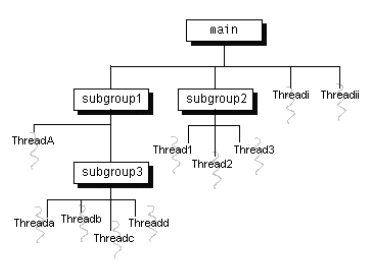
\includegraphics[width=8cm]{images/thread-groups.png}}}
                \caption{Representaci\'on de los grupos de Threads.}
            \end{figure}
	    \end{center}
	\end{frame}

    \begin{frame}
		\frametitle{Threads}
		\framesubtitle{Grupos de threads}

        \begin{block}{Grupos de threads} 
            Para conseguir que un \textbf{thread} pertenezca a un grupo concreto, hay que indicarlo al crear el nuevo thread, seg\'un uno de los siguientes constructores:
            \begin{itemize}
                \item[] \textbf{public} Thread (\textbf{ThreadGroup} grupo, \textbf{Runnable} destino)
                \item[] \textbf{public} Thread (\textbf{ThreadGroup} grupo, \textbf{String} nombre)
                \item[] \textbf{public} Thread (\textbf{ThreadGroup} grupo, \textbf{Runnable} destino, \textbf{String} nombre)
            \end{itemize}
        \end{block}
	\end{frame}

    \begin{frame}
		\frametitle{Threads}
		\framesubtitle{Grupos de threads}

        \begin{block}{Grupos de threads} 
            A su vez, un \textbf{ThreadGroup} debe pertenecer a otro \textbf{ThreadGroup}. Como ocurr\'ia en el caso anterior, si no se especifica ninguno, el nuevo grupo pertenecer\'a al \textbf{ThreadGroup} desde el que ha sido creado (por defecto al grupo \textbf{main}). La clase \textbf{ThreadGroup} tiene dos posibles constructores: 
            \begin{itemize}
                \item[] \textbf{public} ThreadGroup (\textbf{ThreadGroup} parent, \textbf{String} nombre)
                \item[] \textbf{public} ThreadGroup (\textbf{String} nombre)
            \end{itemize}
        \end{block}
	\end{frame}

    \begin{frame}
		\frametitle{Preguntas}

		\hspace{4cm}\huge{Preguntas ?}
		
	\end{frame}
	
    \begin{frame}
		\frametitle{Threads}
		\framesubtitle{Ejercicio}

        \begin{exampleblock}{Ejercicio} 
            {\scriptsize
            Simular el proceso de cobro de un supermercado; unos clientes van con un carro lleno de productos y una cajera les cobra los productos, pas\'andolos uno a uno por el esc\'aner de la caja registradora. En este caso la cajera debe de procesar la compra cliente a cliente, es decir que primero le cobra al cliente 1, luego al cliente 2 y as\'i sucesivamente. Para ello vamos a definir una clase ''\textbf{Cajera}'' y una clase ''\textbf{Cliente}'' el cual tendr\'a un ''array de enteros'' que representar\'an los productos que ha comprado y el tiempo que la cajera tardar\'a en pasar el producto por el esc\'aner; es decir, que si tenemos un array con \textbf{[1,3,5]} significar\'a que el cliente ha comprado 3 productos y que la cajera tardara en procesar el producto 1 \textbf{'1 segundo'}, el producto 2 \textbf{'3 segundos'} y el producto 3 en \textbf{'5 segundos'}, con lo cual tardar\'a en cobrar al cliente toda su compra \textbf{'9 segundos'}.
            }
        \end{exampleblock}
	\end{frame}	

    \begin{frame}
		\frametitle{Threads}
		\framesubtitle{Ejercicio}

        \begin{exampleblock}{Ejercicio} 
            {\scriptsize
            Simular el proceso de parking o estacionamiento que pose\'e una \'unica entrada y una \'unica salida. La idea es controlar el ingreso y egreso de aut\'omoviles, de tal manera que no sea factible el ingreso de un nuevo veh\'iculo si el estacionamiento est\'a lleno y no es factible sacar un aut\'omovil si el estacionamiento est\'a vac\'io. Considere como \textbf{regi\'on cr\'itica} el n\'umero actual de veh\'iculos en el estacionamiento, por lo cual debe utilizar \textbf{bloqueos/sincronizaci\'on de thread}.
            }
        \end{exampleblock}
	\end{frame}	
	
	\begin{frame}
		\frametitle{Threads}
		\framesubtitle{Ejercicio}

        \begin{exampleblock}{Ejercicio} 
            {\scriptsize
            Simular el proceso de deposito y giro de dinero de una cuenta corriente. La idea es controlar el ingreso y egreso de dinero, de tal manera que no sea factible girar dinero si la cuenta est\'a en valor negativo y no sea factible mantener m\'as de \$100.000 (cien mil pesos) en la cuenta. Cada transaci\'on debe esperar un n\'umero aletorio de segundos (entre 1 y 5) y el monto a depositar o girar tambi\'en deber\'a ser aleatorio entre \$1.000 (mil) y \$10.000 (diez mill). Considere como \textbf{regi\'on cr\'itica} la clase que gestiona la cuenta corriente (el saldo), por lo cual debe utilizar \textbf{bloqueos/sincronizaci\'on de thread}.
            }
        \end{exampleblock}
	\end{frame}		
\end{document}

\usetheme{default}
\usetheme{JuanLesPins}
\usetheme{Goettingen}
\usetheme{Szeged}
\usetheme{Warsaw}

\usecolortheme{crane}

\usefonttheme{serif}
\usefonttheme{structuresmallcapsserif}
